\documentclass[11pt]{article}
\usepackage{multicol}
\usepackage{graphicx}
\usepackage{todonotes}
\usepackage{tcolorbox}

\usepackage{anysize,color,float,graphicx,url,comment,hyperref,ulem}
\usepackage{hyperref}
\hypersetup{
    colorlinks=true,
    linkcolor=blue,
    filecolor=magenta,      
    urlcolor=red,
}
\usepackage{amsmath, amsfonts, amssymb}
\usepackage{enumitem}
\usepackage{HW}
\includecomment{comment}
\excludecomment{studentSpace}
\includecomment{studentSpace}

\includecomment{answer}
\excludecomment{answer}
\includecomment{comment}
\newcommand{\blank}{
\underline{\hspace{1.5cm}\hspace{1.5cm}}
}
\newcommand{\norm}[1]{\left\lVert#1\right\rVert}

\begin{document}
\titleline{\semester}
\exhead{Problem Set: Due: 10:00 PM,  18-Feb}
\begin{itemize}
\item Please write (only if true) the honor code. If you used any
  source (person or thing) explicitly state it. 

\item Important: This is an INDIVIDUAL assignment.

\item Always provide a brief explanation. (The length of the
  explanation required has been forecasted with the amount of space
  provided.)
  
\item Submit following files in folder name lab03\_roll\_XX :
	\begin{enumerate}
      \item readme.txt (case sensitive name). This \emph{text} file
        contains identifying information, honor code, links to
        references used 
      \item ReflectionEssay.pdf is optional but a brief one would be nice.
      \item lab03\_roll\_XX.pdf (includes all solutions). 
      \item All relevant tex source (and images only if necessary). No
        other junk files, please.
     \end{enumerate}
\end{itemize} 

\hrulefill
\begin{enumerate}

\begin{tcolorbox}
\item  State whether or not the following points are the same and explain why.
\begin{multicols}{2}
\begin{enumerate}[]
\item
$A[2, -1, 3]$, $B[4,-2,6]$
\item
$A[\sqrt{2}/2, -1,0]$, $B[1,-\sqrt{2},0]$
\end{enumerate}
\end{multicols}
\begin{studentSpace}
\vspace{3cm}
\end{studentSpace}

\end{tcolorbox} \begin{tcolorbox}
\item In projective three-space, what are the standard homogeneous
  coordinates of (a) the origin and (b) ideal points determined by the
  intersections of the extensions of the coordinate axes and the ideal
  plane?


\begin{studentSpace}
\vspace{3cm}
\end{studentSpace}
\end{tcolorbox}

\begin{tcolorbox}
\item Write standard homogeneous coordinates for the points specified
  in uppercase characters. (Use left and right to distinguish.)

\begin{minipage}{0.45\textwidth}
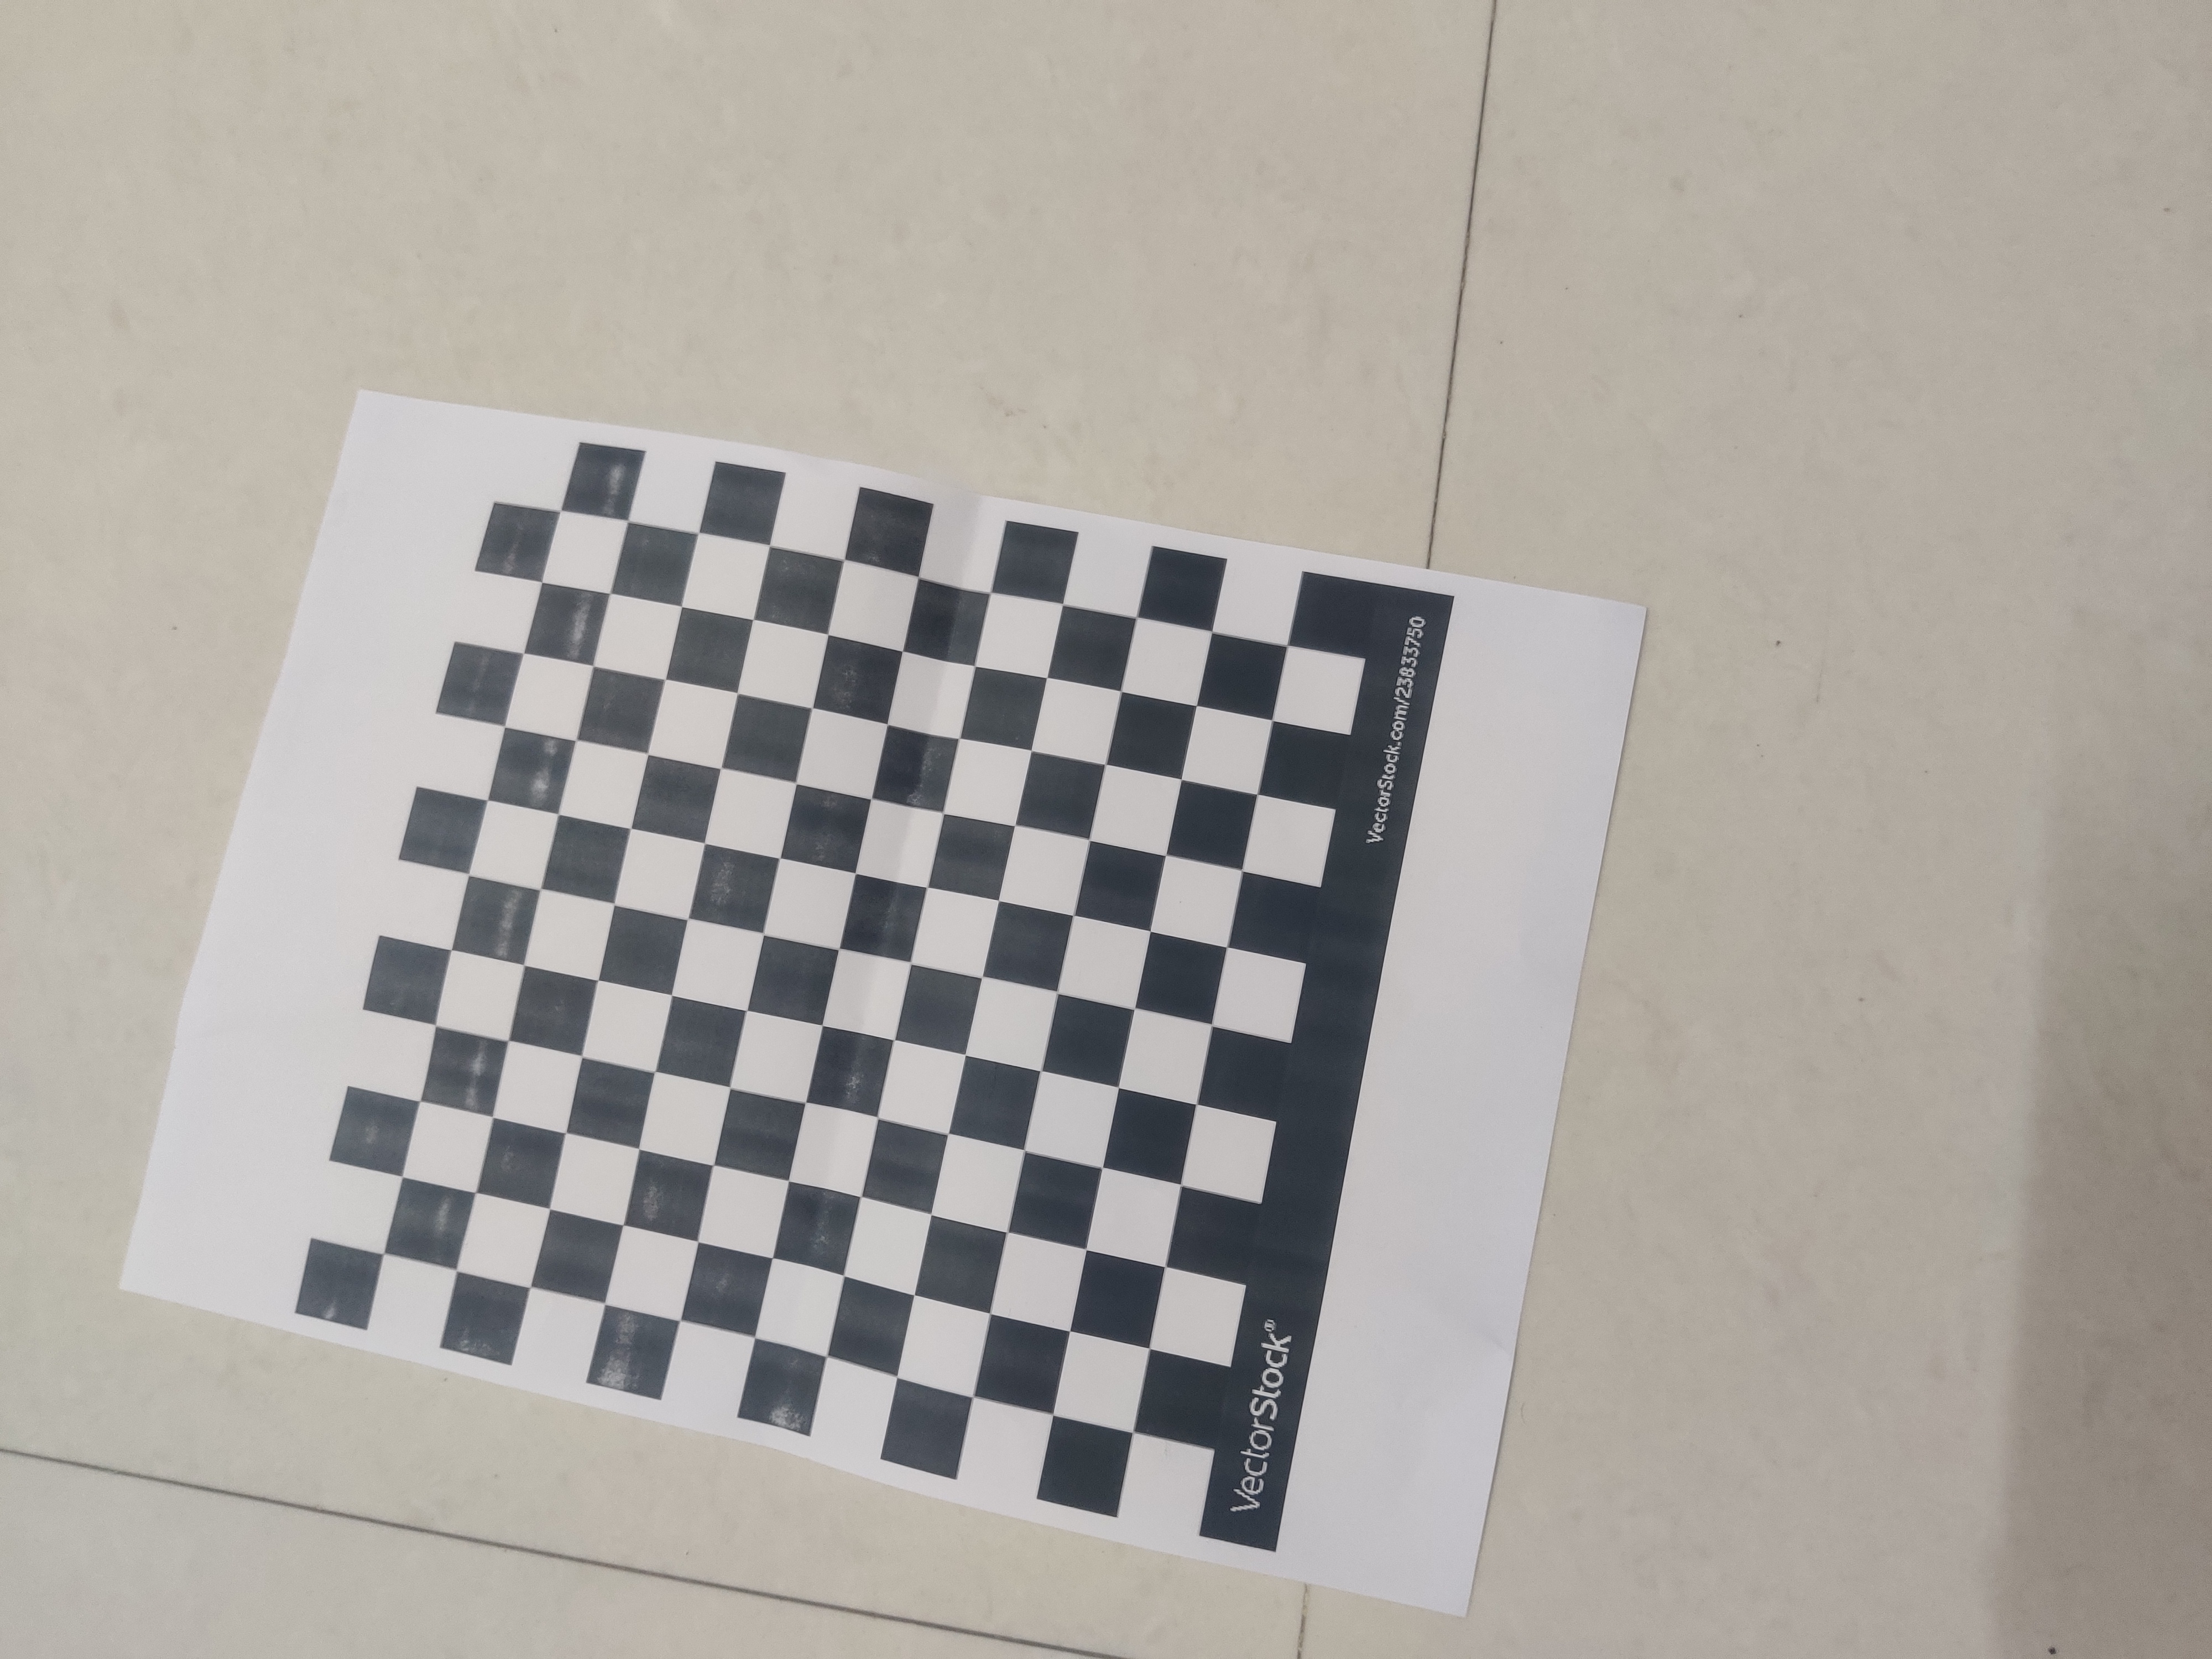
\includegraphics[width=\textwidth, height=.5\textheight,keepaspectratio]{images/image2.png}
\end{minipage} \hfill
\begin{minipage}{0.45\textwidth}
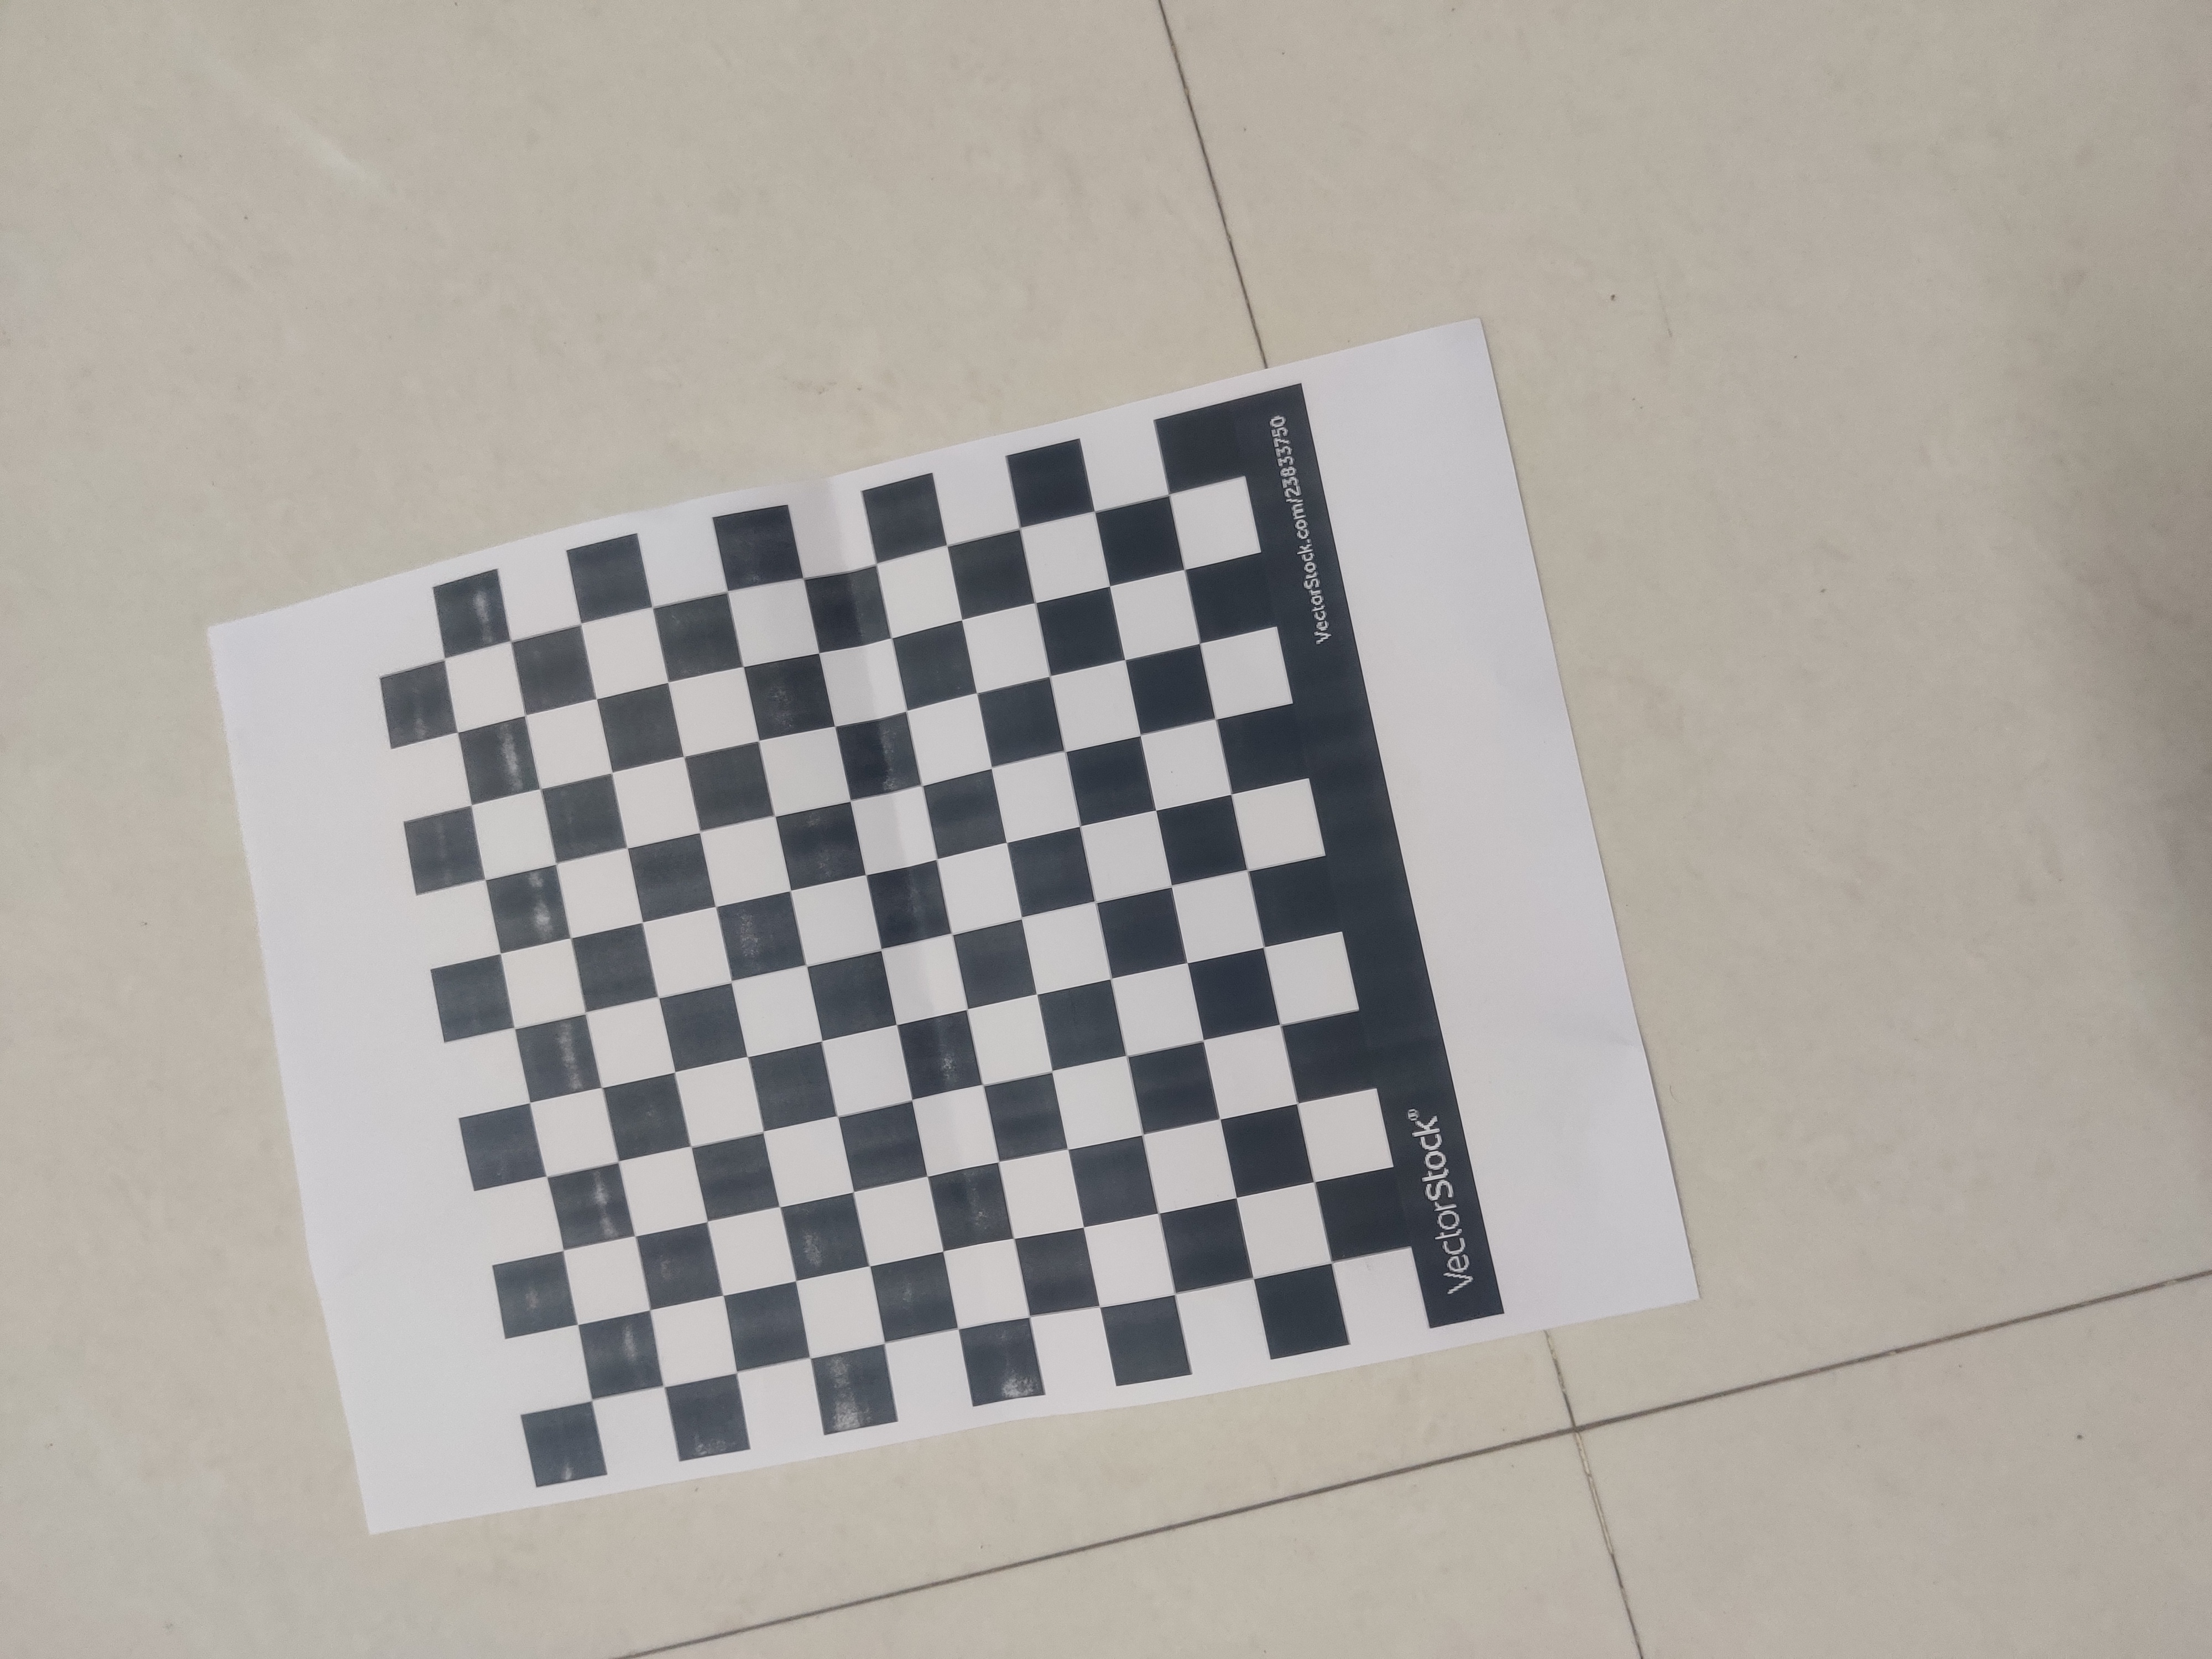
\includegraphics[width=\textwidth, height=.5\textheight,keepaspectratio]{images/image1}
\end{minipage}

\begin{studentSpace}
\vspace{3cm}
\end{studentSpace}



\end{tcolorbox} \begin{tcolorbox}
\item Which of the following points lie on the line $3p_1 -2p_2+5p_3 =
  0$?  Why?
\begin{multicols}{2}
\begin{enumerate}[]
\item
$A[1,1,2]$
\item
$B[4,1,-2]$
\end{enumerate}
\end{multicols}
\begin{studentSpace}
\vspace{3cm}
\end{studentSpace}

\end{tcolorbox} \begin{tcolorbox}
\item Write the coordinates of the lines that are the extensions to the
  projective plane of the following Euclidean lines.
\begin{multicols}{2}
\begin{enumerate}[]
\item
$3x + 2y = 6$
\item
$4x + 5y + 7 = 0$
\end{enumerate}
\end{multicols}
\begin{studentSpace}
\vspace{3cm}
\end{studentSpace}

\end{tcolorbox} \begin{tcolorbox}
\item Sketch each line in the projective plane whose equation is given.
\begin{multicols}{2}
\begin{enumerate}[]
\item
$2p_1 + 3p_2 + 5p_3 = 0$
\item
$3p_1 - 2p_2 - p_3 = 0$
\end{enumerate}
\end{multicols}
\begin{studentSpace}
\vspace{6cm}
\end{studentSpace}


\end{tcolorbox} \begin{tcolorbox}
\item  In each of the following cases, sketch the line determined by the two given points; then find the equation of the line.
\begin{multicols}{2}
\begin{enumerate}[]
\item
$A[3, 1, 2]$, $B[1,2,-1]$
\item
$A[2,1,3]$, $B[1,2,0]$
\end{enumerate}
\end{multicols}
\begin{studentSpace}
\vspace{6cm}
\end{studentSpace}


\end{tcolorbox} \begin{tcolorbox}
\item  Find the standard homogeneous coordinates of the point of
  intersection for each pair of lines. 
\begin{multicols}{2}
\begin{enumerate}[]
\item
$p_1 + p_2 - 2p_3 = 0, 3p_1 + p_2 + 4p_3 = 0$
\item
$p_1 + p_2 = 0, 4p_1 - 2p_2 + p_3 = 0$
\end{enumerate}
\end{multicols}
\begin{studentSpace}
\vspace{3cm}
\end{studentSpace}


\end{tcolorbox} \begin{tcolorbox}
\item  Determine which of the following sets of three points are collinear. 
\begin{multicols}{2}
\begin{enumerate}[]
\item
$A[1,2,1]$, $B[0,1,3]$, $[2,1,1]$
\item
$A[1,2,3]$, $B[2,4,3]$, $[1,2,-2]$
\end{enumerate}
\end{multicols}
\begin{studentSpace}
\vspace{6cm}
\end{studentSpace}

\end{tcolorbox} \begin{tcolorbox}
\item  Determine which of the following sets of three lines meet in a
  point. 
\begin{multicols}{2}
\begin{enumerate}[]
\item
$l[1,0,1], m[1,1,0], n[0,1,-1]$
\item
$l[1,0,-1], m[1,-2,1], n[3,-2,-1]$
\end{enumerate}
\end{multicols}
\begin{studentSpace}
\vspace{6cm}
\end{studentSpace}
\end{tcolorbox}

\end{enumerate}
\end{document}

